\section{Introduction}

We use the awesome apa6 / apa7 package (from Brian D. Beitzel \& Daniel A. Weiss) to create a beatiful APA-style manuscript. Let's cite \textcite{Michel2021} to showcase how citation commands are used \parencite[also works in parentheses, see][]{Michel2021}. Figure \ref{fig:fig1} shows an APA figure example.


\begin{figure}[!ht]
    \centering
    \caption{}
    \label{fig:fig1}
    \caption*{\textit{APA Requires The Title Above The Figure}}
    \vspace*{8mm}
    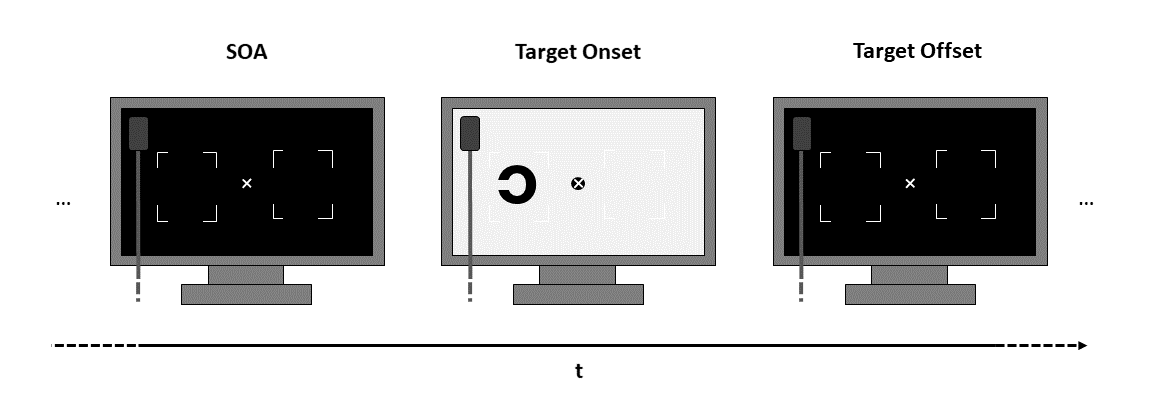
\includegraphics[width=1\textwidth]{../figures/Fig1}
    \caption*{\textit{Note.} Here you can add all your notes regarding the figure.}
\end{figure}
